\documentclass{standalone}
\usepackage[dvipsnames]{xcolor}

\usepackage{tikz}
\usetikzlibrary{chains,scopes}
\usetikzlibrary{decorations.pathreplacing,shapes}
\usetikzlibrary{shapes.multipart}
\usetikzlibrary{arrows}

\begin{document}
	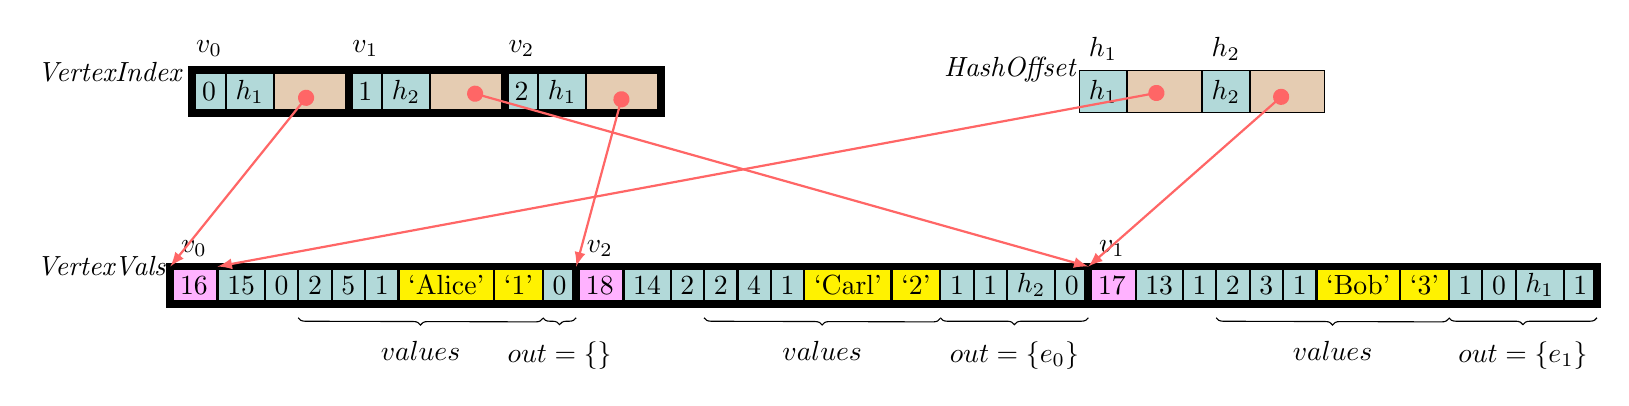
\begin{tikzpicture}
	
	%%% VertexVals
	\begin{scope}[start chain,node distance=0cm]
	\node[label=above:{$v_0$},draw,fill=Fuchsia!30,on chain] (a) at (-1,0) {16};
	\node[draw,fill=teal!30,on chain] (b) {15};
	\node[draw,fill=teal!30,on chain] (c) {0};
	\node[draw,fill=teal!30,on chain] (d) {2};
	\node[draw,fill=teal!30,on chain] (e) {5};
	\node[draw,fill=teal!30,on chain] (f) {1};
	\node[draw,fill=yellow,on chain] (g) {`Alice'};
	\node[draw,fill=yellow,on chain] (h) {`1'};
	\draw [decoration={brace,mirror,raise=5pt},decorate] (d.south west) --  node[below=10pt]{$values$}(h.south east); 
	\node[draw,fill=teal!30,on chain] (l) {0};
	\draw [decoration={brace,mirror,raise=5pt},decorate] (l.south west) --  node[below=10pt]{$out=\{\}$}(l.south east); 
	
	%%%
	\node[label=above:{$v_2$},draw,fill=Fuchsia!30,on chain] (a2) {18};
	\node[draw,fill=teal!30,on chain] (b2) {14};
	\node[draw,fill=teal!30,on chain] (c2) {2};
	\node[draw,fill=teal!30,on chain] (d2) {2};
	\node[draw,fill=teal!30,on chain] (e2) {4};
	\node[draw,fill=teal!30,on chain] (f2) {1};
	\node[draw,fill=yellow,on chain] (g2) {`Carl'};
	\node[draw,fill=yellow,on chain] (h2) {`2'};
	\draw [decoration={brace,mirror,raise=5pt},decorate] (d2.south west) --  node[below=10pt]{$values$}(h2.south east);
	\node[draw,fill=teal!30,on chain] (j2) {1};
	\node[draw,fill=teal!30,on chain] (k2) {1};
	\node[draw,fill=teal!30,on chain] (l2) {$h_2$};
	\node[draw,fill=teal!30,on chain] (m2) {0};
	\draw [decoration={brace,mirror,raise=5pt},decorate] (j2.south west) --  node[below=10pt]{$out=\{e_0\}$}(m2.south east); 
	
	%%%
	\node[label=above:{$v_1$},draw,fill=Fuchsia!30,on chain] (a1) {17};
	\node[draw,fill=teal!30,on chain] (b1) {13};
	\node[draw,fill=teal!30,on chain] (c1) {1};
	\node[draw,fill=teal!30,on chain] (d1) {2};
	\node[draw,fill=teal!30,on chain] (e1) {3};
	\node[draw,fill=teal!30,on chain] (f1) {1};
	\node[draw,fill=yellow,on chain] (g1) {`Bob'};
	\node[draw,fill=yellow,on chain] (h1) {`3'};
	\draw [decoration={brace,mirror,raise=5pt},decorate] (d1.south west) --  node[below=10pt]{$values$}(h1.south east);
	\node[draw,fill=teal!30,on chain] (l1) {1};
	\node[draw,fill=teal!30,on chain] (m1) {0};
	\node[draw,fill=teal!30,on chain] (n1) {$h_1$};
	\node[draw,fill=teal!30,on chain] (o1) {1};
	\draw [decoration={brace,mirror,raise=5pt},decorate] (l1.south west) --  node[below=10pt]{$out=\{e_1\}$}(o1.south east); 
	
	
	%%%
	\end{scope};
	
	    %% Bordi VertexVals
		\draw[draw,line width=1mm] (a.south west) rectangle (l.north east);
		\draw[draw,line width=1mm] (a1.south west) rectangle (o1.north east);
		\draw[draw,line width=1mm] (a2.south west) rectangle (m2.north east);
	
	%% HashOffset
		\begin{scope}[start chain,node distance=0cm,xshift=300,yshift=70,minimum height=1.5em]
		\node[label=above:{$h_1$},draw,fill=teal!30,on chain] (h1) {$h_1$};
		\node[draw,fill=brown!40,on chain] (p1) {$\qquad$};
		\node[label=above:{$h_2$},draw,fill=teal!30,on chain] (h2) {$h_2$};
		\node[draw,fill=brown!40,on chain] (p2) {$\qquad$};
		%\draw[draw,line width=1mm] (v1.south west) rectangle (pv1.north east);
		%\draw[draw,line width=1mm] (v2.south west) rectangle (pv2.north east);
		
		%% Frecce HashOffset
		\draw[*-latex,red!60,thick] (p2.center) -- (a1.north west);
		\draw[*-latex,red!60,thick] (p1.center) -- (b.north west);
		\end{scope};
	
%% VertexIndex
\begin{scope}[start chain,node distance=0cm,yshift=70,xshift=-23,minimum height=1.5em]
\node[label=above:{$v_0$},draw,fill=teal!30,on chain] (v1) {$0$};
\node[draw,fill=teal!30,on chain] (hx) {$h_1$};
\node[draw,fill=brown!40,on chain] (pv1) {$\qquad$};

\node[label=above:{$v_1$},draw,fill=teal!30,on chain] (v2) {$1$};
\node[draw,fill=teal!30,on chain] (h2) {$h_2$};
\node[draw,fill=brown!40,on chain] (pv2) {$\qquad$};
\node[label=above:{$v_2$},draw,fill=teal!30,on chain] (v3) {$2$};
\node[draw,fill=teal!30,on chain] (h3) {$h_1$};
\node[draw,fill=brown!40,on chain] (pv3) {$\qquad$};
\end{scope};

%% Rettangoli di bordo
\draw[draw,line width=1mm] (v1.south west) rectangle (pv1.north east);
\draw[draw,line width=1mm] (v2.south west) rectangle (pv2.north east);
\draw[draw,line width=1mm] (v3.south west) rectangle (pv3.north east);

%% Frecce VertexIndex
\draw[*-latex,red!60,thick] (pv1.center) -- (a.north west);
\draw[*-latex,red!60,thick] (pv2.center) -- (a1.north west);
\draw[*-latex,red!60,thick] (pv3.center) -- (a2.north west);

\node[left=25 pt of a.west,anchor=south,font=\itshape] {VertexVals};
\node[left=30 pt of v1.west,anchor=south,font=\itshape] {VertexIndex};
\node[left=25 pt of h1.west,anchor=south,font=\itshape] {HashOffset};
	\end{tikzpicture}
	
\end{document}